\documentclass[a4paper,10pt]{report}

\usepackage[in]{fullpage}
\usepackage{parskip}
\usepackage{tikz}
\usepackage{amsmath}
\usepackage[backend=bibtex,style=numeric-comp,sorting=nyt,sortcites=true]{biblatex}
\usepackage[section]{placeins}
\usepackage[color]{circus}
\usepackage{fixltx2e}

\title{Qualifying Dissertation}
\author{James Baxter}
\date{}

\bibliography{literature} 

%TC:group zed 0 displaymath
%TC:group axdef 0 displaymath
%TC:group schema 1 displaymath
%TC:group circus 0 displaymath
%TC:group circusaction 0 displaymath

\begin{document}
\maketitle

%TODO: abstract

\tableofcontents

\chapter{Introduction}

This section begins by explaining the motivation for the work decribed in
this report. Then the objectives of the work, which come from the motivation,
are described and, finally, the structure of the remainder of this report is
described.

\section{Motivation}

Since its release in 1995, the Java programming language~\cite{gosling2013} has
increased in popularity and is now used on a wide variety of platforms.  This
popularity means that Java has been used in a wide variety of areas including
desktop applications, on the internet in the form of Java applets, on
smartcards~\cite{chen2000} and on mobile devices~\cite{oracle2014}.  Several
languages derived from Java have also been created, including
Scala~\cite{lausanne2015} and Ceylon~\cite{redhat2015}, as well as older
variants of Java such as MultiJava~\cite{clifton2006} and
Pizza~\cite{odersky1997}, which have in turn contributed to the development of
Java. Scala adds functional programming features to Java, some of which have
been incorporated into Java 8. Ceylon extends Java's type system with features
such as union types, correcting some common Java errors in the process.
% add a short sentence describing each langauage, try to find more non-webpage references

One use of Java that is of particular interest is its use in embedded systems.
While early versions of Java were developed with the intention of using them on
embedded systems, particularly TV set-top boxes, the technology was not well
received and it was only in the growing sector of the internet that Java
intitially found a market. % need citation for this - horstmann2002?
However, it was soon realised that the portability, modularity, safety and
security benefits of Java could be of great use in embedded
systems. % need citation for this
This required the creation of specialised Java virtual machines as the standard
JVM is too large for most embedded systems and much research has gone into
making increasingly smaller virtual machines to increase the range of devices
that Java can be used on~\cite{caska2011,thomm2010}.

Many embedded systems are also real-time systems, but features of Java such as
the garbage collector and the concurrency model make it unsuitable for real-time
systems, where strict guarantees about timing properties must be made.  To
rectify these problems the Real-Time Specification for Java
(RTSJ)~\cite{gosling2000} was created.  The RTSJ extends Java with a scoped
memory model and a more predictable scheduling system, which allow RTSJ programs
to fulfil real-time requirements.

While the RTSJ addresses real-time requirements of embedded systems, many
embedded systems are also safety-critical.  Safety-critical programs must
usually be shown to conform to certain standards of safety such as,
\mbox{DO-178C} and ISO~26262, and so must be amenable to static analysis in
order to determine if they meet the required standards.  To support the
development of safety-critical programs that meet these requirements in Java,
the Safety-Critical Java (SCJ) specification~\cite{locke2013} has been created.
SCJ is a subset of the RTSJ that contains only the features that can be
statically reasoned about, which means that features such as the
garbage-collected heap and dynamic class loading are absent from SCJ.  This
facilitates the creation of SCJ programs that fulfil formal specifications;
indeed work has already been done on developing correct SCJ programs from formal
specifications~\cite{cavalcanti2011, cavalcanti2013}.

While it can be shown that SCJ programs are correct, it must still be ensured
those programs will be run correctly.  In the case of Java this generally means
ensuring the Java compiler and Java Virtual Machine (JVM) are correct. 

Work has been done in the the past on modelling virtual machines for Java, and
on the formal correctness of compilers targetting those virtual machines.  Some
of the most complete work in that area was by St\"{a}rk, Schmid and
B\"{o}rger~\cite{stark2001}, who present a model of the full Java language and
virtual machine, along with a formally verified compiler, although for an older
version of Java than is current.  Other work has also been done on modelling the
JVM and Java compilation using refinement
techniques~\cite{duran2010}. Additionally there has been work considering
machine checked models of Java virtual machines and
compilers~\cite{lochbihler2012, nipkow2000, strecker2002}. Work has also been
done apart from consideration of Java compliers on the semantics of Java
bytecode and verification of standard JVMs~\cite{bertelsen2000, jones1998}.

However, SCJ has a number of differences from standard Java. Firstly, the SCJ
memory model is rather different to the standard Java memory model, abandoning
the garbage collector in favour of a scoped memory model.  Garbage collection is
less predictable and often quite complex, and so difficult to reason about and
unsuitable for some of the strictest certifiability requirements of
safety-critical systems.  By contrast, the scoped memory model provides greater
predictability on when memory is freed as it can be determined when a particular
scope has been left.  Similarly, the SCJ approach to scheduling differs from
that of standard Java, using a preemptive priority scheduling approach rather
than the unpredictable scheduling of standard Java threads.  These differences
of SCJ from standard Java mean that the standard JVM is not suitable for running
SCJ programs.  A specialised virtual machine is required and the specialised
virtual machine must also be verified.

In the case of virtual machines for embedded systems, the priorities are usually
size and speed, which generally results in machines that are hard to verify.  In
any case, virtual machines that rely on interpreting bytecode are unsuitable for
real-time embedded systems as they are likely to be slower than running native
code directly.

An alternative method to run a Java program is to compile it to native code and
some authors have suggested doing so either directly~\cite{schultz2003} or via
C~\cite{varma2004}. There are also several virtual machines that take this
approach including Fiji VM~\cite{pizlo2009}, Icecap HVM~\cite{sondergaard2012}
and OVM~\cite{armbruster2007}.  This allows correct running of an otherwise
correct SCJ program to be viewed as a compiler verification problem.

There has been much research in the past into compiler correctness as correct
compilation is important to the correct functioning of a program, even when the
program itself has been shown to be correct.  Much of the work follows a
commuting diagram approach, in which the compilation is shown to be consistent
with transformation between the semantics of the source and target
languages\cite{morris1973, thatcher1979}. This approach is apparent in much of
the early work such as that of McCarthy and Painter~\cite{mccarthy1967}, as well
as in more recent work such as the CompCert project~\cite{leroy2009a,
  leroy2009b}. There has also been work done using this approach in automated
theorem provers~\cite{klein2006, milner1972, nipkow2000}, which provide
additional certainty that the proof is correct and can also provide code
generation facilities to allow creation of a working compiler.

An alternative approach to compiler verification is the algebraic
approach~\cite{hoare1991, sampaio1993}, based on modelling compilation using
refinement calculus~\cite{back1981, morgan1990, morris1987}. This approach
appears to be less commonly used but has been applied to Java~\cite{duran2005,
  duran2010} and hardware description languages~\cite{perna2010,
  perna2011}. This approach is also quite amenable to automation as it relies on
refinement laws that can be applied by a term rewriting system.

There is a clear need for formal verification of SCJ virtual machines due to the
safety-critical nature of the systems involved and the fact that safety
standards such as DO-178C require it at the highest safety levels. However,
there appears to be little work done in that area and no known SCJ virtual
machines have been formally verified.

% explain that there is a gap with no verification for SCJ compilers for embedded systems

\section{Objectives}

Given that there is a need for a formally verified virtual machine that can run
SCJ programs efficiently on an embedded system, my objective is to identify the
requirements of such a virtual machine. These requirements will be expressed in
formal notation so as to permit proofs of correctness, and allow verification
and construction of provably correct virtual machines.

As many existing SCJ virtual machines, particularly those targetting embedded
systems, take the approach of compiling Java bytecode to native code in order to
improve speed, formal specification of a SCJ virtual also includes the
specification and verification of such a compiler. This must be done in addition
to ensuring the virtual machine caters for the requirements of SCJ with regard
to areas such as scheduling and memory management.

\section{Document Structure}

Having given a brief overview of the area of study and identified the problem we
wish to consider, the remainder of this report will proceed as follows: 

In Chapter~\ref{literature-review-chapter} we will examine the literature on
safety-critical virtual machines and compilers for Java-like languages. This
includes a discussion of why a safety-critical variant of Java is necessary and
how it differs from standard Java so as to make a specialised virtual machine
necessary, followed by a survey of the existing virtual machines for
Saftey-Critical Java and the techniques used in verifying compilers.

Then, in Chapter~\ref{research-proposal-chapter} we will cover the structure and
plan for the proposed research.

In Chapter~\ref{requirements-chapter} we will present some
preliminary results identifying the requirements of an SCJ virtual machine, with
a formal model of those requirements in the \Circus{} specification language in
Section~\ref{formal-model-section}.

Finally, we conclude in Chapter~\ref{conclusions-chapter} by mentioning some
related work and the wider context of this research.

% Description of SCJ and review of SCJ VMs - use stuff from JTRES paper, maybe extend it a bit
% Review the literature on compiler correctness 
%  - Two approaches: algebraic and commuting diagram
%  - Consider each approach in a separate subsection and compare them
%  - Make sure to descibe the *approach* in detail, not what the authors did
%  - Finish by looking at and comparing some of the work on Java compilation
% Present research proposal and preliminary results
% - Overall plan - requirements for an SCJVM - explain different parts of the diagram, mention CEE will be dealt with by later work
% - Present the identification of the requirements for the VM services from the JTRES paper
% - Discuss the formal model - similar to JTRES paper but room to go into more depth


\chapter{Compilers and Virtual Machines for Java-like languages in the
  Safety-critical Domain}
\label{literature-review-chapter}

\section{Java for Safety-critical systems}
% provide motivation for SCJ, mentioning standard Java and RTSJ

\section{Safety-Critical Java}
\label{scj-sec}

Safety-Critical Java is a variant of Java designed for writing Java programs
where certifiability is an important concern.  SCJ is based upon the Real-Time
Specification for Java, which augments the standard Java scheduler and
gar\-bage-collected heap with more predictable priority-scheduled event handlers
and scoped memory areas.  The modification that SCJ makes to the RTSJ is to
remove the aspects of RTSJ that make certification difficult, including removal
of standard Java threads and the garbage collector.  This leaves scheduling and
memory management models that are very different to the models for standard Java
and that, therefore, require specialised virtual machines to support them.

An SCJ program consists of one or more missions, which are collections of
schedulable objects that are scheduled by SCJ's priority scheduler. Missions are
run in an order determined by the mission sequencer supplied by an SCJ
program. Running a mission consists of starting each of the schedulable objects
in the mission, waiting for a request to terminate the mission, then terminating
each of the schedulable objects in the mission.  The schedulable objects within
a mission are event handlers that are released either periodically, at set
intervals of time, aperiodically, in response to a release request from a
hardware interrupt or another handler, or once at a specific point in time
(though handlers that are released once can have a new release time set,
allowing them to be released again).

Each schedulable object has a priority and the highest priority object that is
eligible to run at each point in time are the objects that run. This allows for
simpler reasoning about order of execution and allows for more urgent tasks to
preempt less urgent tasks.

SCJ allows for assigning schedulable objects to ``scheduling allocation
domains'', where each domain consists of one or more processors.  At Level 1,
each scheduling allocation domain is restricted to a single processor.  Hence,
in scheduling terms, the system is fully partitioned. This allows for mature
single processor schedulability analysis to be applied to each domain, although
the calculation of the blocking times when accessing global synchronised methods
will be different than they would be on a single processor system due to the
potential for remote blocking~\cite{davis2011}.

SCJ deals with memory in terms of memory areas, which are Java objects that
provide an interface to blocks of physical memory called backing stores.  Memory
allocations in SCJ are performed in the backing store of the memory area
designated as the allocation context.  Each schedulable object has a memory area
associated with it that is used as the allocation context during a release of
that object, and is cleared after each release.  Each mission also has a mission
memory area that can be used as an allocation context by the schedulable objects
of that mission, to provide space for objects that persist for the duration of
the mission or that need to be shared between the schedulable objects.  There is
also an immortal memory area where objects can be allocated that will be needed
for the entire running of the program (and so will never be freed).

This system of memory areas makes it easy to predict when memory will be freed,
which cannot be easily done with a garbage-collected heap.  Furthermore, this
memory model cannot be achieved with a standard JVM as it does not provide
memory outside of the heap for allocation and lacks a notion of allocation
context. The memory manager should also provide a means of accessing raw memory
for the purposes of device access, but that section of the SCJ standard is not
yet finalised so we will not cover it here. It can, however, be seen that any
system of raw memory access is not supported by most standard JVMs.

A further requirement of SCJ is that dynamic class loading is not allowed; all
classes used by the program must be loaded when the program starts. This is
because dynamic class loading may introduce time overheads that are hard to
predict and also introduces additional code paths that complicate the
certification of programs.  SCJ also disallows object finalisers as it is not
always easy to predict when they will be run.

\section{Virtual Machines for Safety-Critical Java}
% one subsection per machine

Because of these features of SCJ, a specialised virtual machine that provides
support for allocation in memory areas and preemptive scheduling is required for
SCJ. Although SCJ is a relatively recent development there have been various
virtual machines created for SCJ or variations of SCJ, including including Fiji
VM~\cite{pizlo2009}, Icecap HVM~\cite{sondergaard2012},
OVM~\cite{armbruster2007}, HVM\textsubscript{TP}~\cite{luckow2014} and PERC
Pico~\cite{atego2015, richard2010}. Most of these are targeted at embedded
systems with real time constraints.

The Fiji VM and Icecap HVM both take the approach of precompiling Java
bytecode to C in order to allow for faster running programs with fewer
memory resources.  Fiji VM is, however, not specifically concerned
with SCJ; it is rather designed to run general real-time Java
programs, though this includes providing support for SCJ.  By
contrast, Icecap has been designed specifically to run SCJ
programs. It includes an implementation of the SCJ libraries, although
they cannot be easily decoupled from the virtual machine itself.

Icecap also provides a lightweight Java bytecode interpreter and
allows for interpreted code to be mixed with compiled
code. HVM\textsubscript{TP} is a modification of the Icecap HVM's
bytecode interpreter to improve time predictability and ensure that
bytecode instructions are executed in constant time.

OVM works on a principle of precompiling code for performance reasons, similar
to Fiji VM and Icecap HVM, but translates Java to C++ instead of bytecode to C.
OVM also differs from the Icecap HVM and Fiji VM in that it predates SCJ. It is
written to implement the Real-Time Specification for Java
(RTSJ)~\cite{gosling2000}, though it can still support SCJ programs as SCJ is
based on a subset of RTSJ.

PERC Pico is a product of Atego based on early ideas for SCJ, but uses its own
system of Java metadata annotations to ensure the safety of scoped memory. PERC
Pico does not support the current SCJ standard.

In summary, as far as I am aware there is one implementation of an SCJ VM
publicly available, which is the Icecap HVM. This is and, typically, virtual
machines for SCJ will be, designed to be very small and fast so as to be able to
run on embedded systems.  While these are important goals in an embedded virtual
machine implementation, the resultant virtual machines tend to be complex and so
hard to verify.  There does not yet appear to be any work on verification of an
SCJ virtual machine.  Moreover, not even the requirements of an SCJ virtual
machine, which must be clearly identified before verification can commence, are
currently agreed on.

\section{Compiler Correctness}
\label{compiler-correctness-sec}

Due to the importance of compiler correctness to the correctness of the programs
produced by it, there has been much research over the years into the area of
compiler correctness. Most of the work done follows a similar approach, which I
will term the commuting diagram approach as it can be viewed as showing that a
particular diagram commutes. I will discuss the commuting diagram approach in
Section~\ref{commuting-diagram-sec}.

An alternative approach to compiler verification is the algebraic approach that
was developed in the early 90s and is based on the concepts of refinement
calculi designed for deriving software from specifications of behaviour. I will
explain the algebraic approach in Section~\ref{algebraic-sec} and discuss how it
differs from the commuting diagram approach.

I will finish in Section~\ref{java-correctness-sec} by reviewing some of the
literature on correctness of compilers for Java-like languages, looking at how
the techniques of compiler correctness have been applied in the case of Java and
comparing the different approaches.

\subsection{Commuting Diagram Approach}
\label{commuting-diagram-sec}

Much of the work on compiler correctness can be seen as following the approach
identified by Lockwood Morris~\cite{morris1973}, and later refined by Thatcher,
Wagner and Wright~\cite{thatcher1979}. The approach is essentially that a
compiler correctness proof should be a proof that the diagram shown in
Figure~\ref{commuting-diagram} commutes, that is, $\gamma \circ \psi = \phi
\circ \epsilon$.

\begin{figure}[ht]
  \begin{center}
    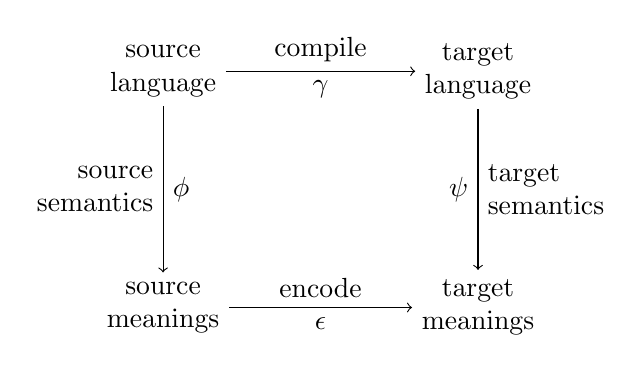
\begin{tikzpicture}
      \node[align=center] (S) at (0cm,3cm) {source\\language};
      \node[align=center] (T) at (4cm,3cm) {target\\language};
      \node[align=center] (M) at (0cm,0cm) {source\\meanings};
      \node[align=center] (U) at (4cm,0cm) {target\\meanings};
      
      \path (S) edge[->] node[align=center, above] {compile}           
        node[align=center, below] {$\gamma$} (T);
      \path (S) edge[->] node[align=right, left]   {source\\semantics} 
        node[align=center, right] {$\phi$} (M);
      \path (T) edge[->] node[align=left, right]   {target\\semantics} 
        node[align=center, left] {$\psi$} (U);
      \path (M) edge[->] node[align=center, above] {encode} 
        node[align=center, below] {$\epsilon$} (U);
    \end{tikzpicture}
  \end{center}
  \caption{The commuting diagram used in the traditional approach to compiler verification}
  \label{commuting-diagram}
\end{figure}

Lockwood Morris had the corners of the diagram as algebras, rather than merely
sets, with the functions between them being homomorphisms in order to add
additional structure to the compiler correctness proof.  This differs from the
approach of some earlier works, particularly the earliest work by McCarthy and
Painter~\cite{mccarthy1967}, and instead follows work such as that of Burstall
and Landin~\cite{burstall1969}.

McCarthy and Painter's work featured a simple expression language with addition,
natural numbers and variables.  This was compiled to a simple 4-instruction
single-register machine. The proof of the compiler's correctness followed the
commuting diagram approach, though the arrows of the diagram were simple
functions rather than homomorphisms and the proof was performed using induction
over the source language. The work is not particularly advanced but did lay the
foundation for the study of compiler correctness.

The approach taken by Burstall and Landin is interesting since, though
they show correctness of a compiler for the same source and target languages as
McCarthy and Painter, they use a more algebraic approach that better matches
what Lockwood Morris later suggested.  Burstall and Landin's approach involved
representing the source and target languages, and their meanings, as algebras,
with the compilation functions as homomorphisms. They then show correctness of
the compilation, targetting several intermediate machines in the
process. Viewing the languages as algebras can be seen to allow for simpler
proofs as some of the arrows of the commuting diagram can be wholly or partially
derived from the algebraic structure. It is this notion of simplifying the
proofs that led Lockwood Morris to advocate the use of algebras and
homomorphisms.

The overall goal of pursuing formal proofs of compiler correctness, as proposed
by McCarthy and Painter~\cite{mccarthy1967}, is to allow machine-checked proofs
of program correctness. There has certainly been work in that area following
McCarthy and Painter's work, the earliest of which is that by Milner and
Weyhrauch~\cite{milner1972} who show the correctness of an ALGOL-like
language. The proof of correctness was partially mechanised in the LCF theorem
prover~\cite{milner1972a} but they were of the opinion that the proof was
feasable and could be completed relatively easily. An interesting point to note
is that Milner and Weyhrauch acknowledged the need for some way of structuring
the proof in order to make it amenable to machine-checking, which gives further
support to the algebraic commuting diagram approach advocated by Lockwood
Morris. Indeed, Milner and Wehrauch explicitly followed that approach as they
were in disscusions with Lockwood Morris.

One advantage to making proofs easily machine-checkable, apart from the added
certainty that the proof is correct, is that working compilers can be created
from the machine-checked proofs via the code generation facitilies available
with many theorem provers such as those of Isabelle/HOL~\cite{haftmann2007} and
Coq~\cite{letouzey2003, letouzey2008}. The fact that the commuting diagram
approach involves treating the compilation as a function between algebras
representing the source and target languages fits well with this idea as there
is then a function defined in the mechanised logic for the purposes of
conducting proofs about it that can be readily extracted to executable code.

The commuting diagram approach has been followed in much of the literature
through the years, though not always with the algebraic methods recommended by
Lockwood Morris.  It seems that the basic structure of the commuting diagram is
a fairly natural approach to take, as seen by work such as that of the ProCoS
project~\cite{buth1992}, which follows the commuting diagram structure although
it does not directly reference the early works advocating an algebraic commuting
diagram approach. Another piece of work that follows the commuting diagram
approach is that of Polak~\cite{polak1981}, who states that he is more
interested in verification of a ``real'' compiler rather than ``abstract code
generating algorithms'', and shows the correctness of a compiler for a
Pascal-like language.  This work also seems to focus much more on pragmatic
applications of the commuting diagram approach, leaving behind the algebraic
ideas of earlier papers (though Polak does cite them) and setting a precedent
for a simpler verification approach based on considering the functions in the
commuting diagram.

The commuting diagram has also been used in recent work, some of the most
successful of which is that of CompCert~\cite{leroy2009a, leroy2009b,
  leroy2012}, which is a project to create a fully verified realistic compiler
for a subset of C, using the theorem prover Coq~\cite{coq2004}.

\subsection{Algebraic Approach}
\label{algebraic-sec}

The second main approach to showing correctness of compilers is the algebraic
approach proposed by Hoare in 1991~\cite{hoare1991}, and further developed by a
student of his~\cite{hoare1993, sampaio1993, sampaio1997}. Note that the
algebraic approach discussed in this section is largely unrelated to the
algebraic commuting diagram approaches mentioned in the previous section.

The algebraic approach to compilation derives from the concepts of algebraic
reasoning about programs and program refinement. These concepts come from the
idea, proposed by Hoare in 1984~\cite{hoare1984}, that programs can be thought
of as predicates and so the laws of predicate logic can be used to construct
laws for reasoning about programs~\cite{hoare1987}. As an example of such a law
for reasoning about programs consider the fact that sequential composition of
programs is associative, as show in Equation~\eqref{seq-comp-assoc}, or the fact
that a program that does nothing, called $\Skip$ here following the \Circus{}
notation, is the identity of sequential composition, as shown in
Equation~\eqref{skip-comp-identity}.
\begin{equation}
  \label{seq-comp-assoc}
  P;(Q;R) = (P;Q);R
\end{equation}
\begin{equation}
  \label{skip-comp-identity}
  P;\Skip = \Skip;P = P
\end{equation}

%TODO: mention some of Bauer's early work on program development by stepwise transformation
The notion of refinement is an important one for the construction of these laws
of programs and the algebraic approach to compilation.  Refinement was
developed, largely independently, by Back~\cite{back1981},
Morris~\cite{morris1987} and Morgan~\cite{morgan1990}.  The basic idea is that
there is a relation between programs that captures the idea of one program being
``at least as good as'' another or, to put it more precisely, at least as
deterministic as another.  The reason for this concept being so important is
that the languages and laws for reasoning about programs can also be used to
develop programs from specifications.  This means that certain things can be
left loosely specified and several different implementations could refine that
specification. % an example of where nondeterminism in a specification is good
               % would be helpful here


\subsection{Correctness of Java Compilers}
\label{java-correctness-sec}

% conclude no efforts to verify SCJVMs, following the normal form approach,
% mention that the VM normal form must be in some specification language to lead
% into the next section

\section{\Circus{}}

% adapt overview of Circus using the clock specification from earlier version of
% JTRES paper

\section{Final Considerations}

% summarise the problem and how to solve it

\chapter{Research Proposal}
\label{research-proposal-chapter}

% Move material from the start of the next chapter to here

\chapter{Requirements of a Safety-Critical Java Virtual Machine}
\label{requirements-chapter}

For the purposes of specification, a Safety-Critical Java virtual machine
(SCJVM) is seen as having the components shown in Figure~\ref{scjvm-fig}. The
SCJVM is spilt into two parts: the core execution environment and the virtual
machine services. The core execution environment handles the running of Java
bytecode.  The virtual machine services support, for example, scheduling and
memory management, that is, services that are required to support the SCJ
infrastructure and the core execution environment.

\begin{figure}[ht]
  \centering
  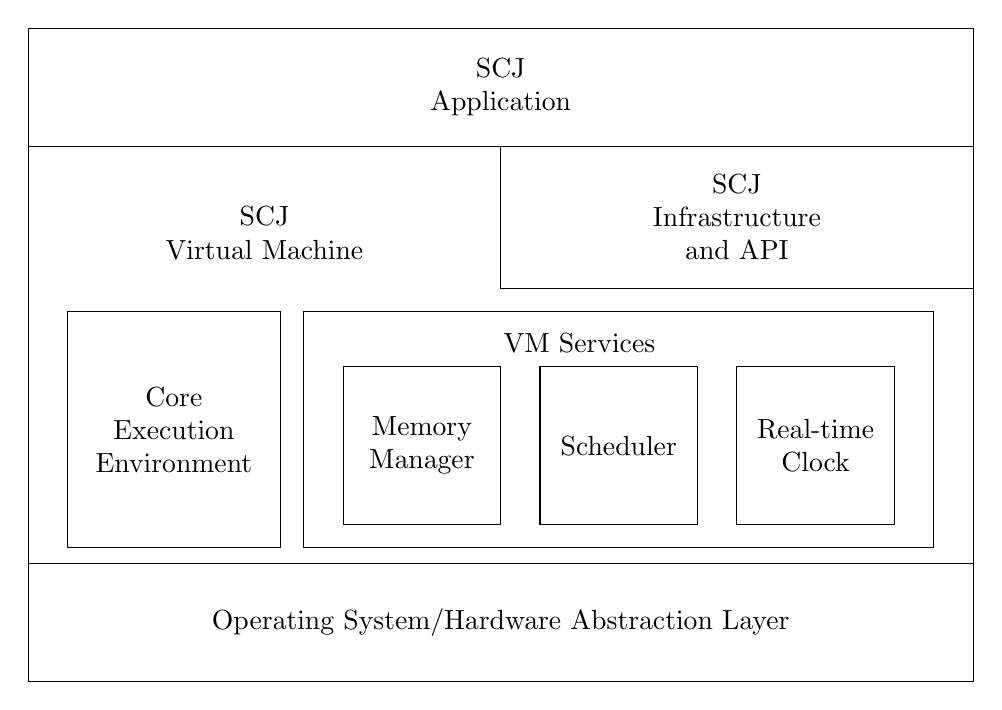
\begin{tikzpicture}
    \draw (0cm,0cm) rectangle (12cm,5.3cm);
    
    \draw (0.5cm,0.2cm) rectangle (3.2cm,3.2cm); \draw (3.5cm,0.2cm) rectangle
    (11.5cm,3.2cm); 
    \foreach \x in {1,...,3} \draw (\x * 2.5cm + 1.5cm,0.5cm)
    rectangle (\x * 2.5cm + 3.5cm,2.5cm) coordinate[pos=0.5](VMService\x);
    
    \node[align=center] at (3cm,4.2cm) {SCJ\\Virtual Machine};
    \node[align=center] at (1.85cm,1.7cm) {Core\\Execution\\Environment};
    \node[align=center] at (7cm,2.8cm) {VM Services}; 
    \node[align=center] at (VMService1) {Memory\\Manager};
    \node[align=center] at (VMService2) {Scheduler};
    \node[align=center] at (VMService3) {Real-time\\Clock};
    
    \draw (0cm,5.3cm) rectangle (12cm,6.8cm) node[pos=0.5,align=center]
    {SCJ\\Application}; \draw (6cm,3.5cm) rectangle (12cm,5.3cm)
    node[pos=0.5,align=center] {SCJ\\Infrastructure\\and API};
    
    \draw (0cm,-1.5cm) rectangle (12cm,0cm) node[pos=0.5,align=center]
    {Operating System/Hardware Abstraction Layer};
  \end{tikzpicture}
  \caption{A diagram showing the structure of the SCJ virtual machine and its
    relation to the SCJ infrastructure and the operating system/hardware
    abstraction layer.}
  \label{scjvm-fig}
\end{figure}

The core execution environment is not necessarily required to use any particular
means to run the bytecode.  It may interpret bytecode instructions, just-in-time
compile the bytecode, or execute native code precompiled from Java bytecode (in
such a case the compiler is regarded as part of the core execution
environment). As many existing virtual machines for SCJ adopt the approach of
compiling to native code, I intend to consider specification of the core
execution environment as specification of a compiler from Java bytecode to
C. The reason for the choice of C as a target language is the same as that of
other SCJ virtual machines: C is a language already widely used in the area of
embedded systems and is sufficiently lightweight to permit its use as a
compilation target.

The approach I will use for specifying and verfying the compilation is the
algebraic approach as it allows for verification to easily flow from
specification without the need for an additional function to verify against as
in the commuting diagram approach. While Java bytecode is the source language of
the compilation, it may be better to have a model of a bytecode interpreter that
resembles the normal form usually used in the algebraic approach and refine it
to a model of C code, essentially applying the algebraic approach in
reverse. The reason for this is that Java bytecode is relatively low-level and
there is a similar model of Java bytecode in Duran's model of Java
compilation. The benefit of having a model of a Java bytecode interpreter is
that it provides a specification of an iterpreter as well as a compiler,
allowing compilation and interpretation to be mixed, as it permitted by the
Icecap HVM. The semantics is not expected differ from the standard semantics of
Java bytecode, except in the instructions relating to scheduling and memory
management, where some changes are envisaged, so the main challenge is in the
compiler verification. It should also be noted that class loading is treated as
part of the core execution environment and so it is bound by the requirement to
load all classes at virtual machine startup.

As can be seen from Figure~\ref{scjvm-fig}, we group the virtual machine
services into three areas:
\begin{itemize}
\item the memory manager, which manages backing stores for memory areas and
  allocation within them;
\item the scheduler, which manages threads and interrupts that allow for
  implementation of SCJ event handlers; and
\item the real-time clock, which provides an interface to the system real-time
  clock.
\end{itemize}
Each of these services is used either by the core execution environment or by
the SCJ infrastructure; some of the services also rely on each other.  For
example, the scheduler must update the allocation context in the memory manager
when performing a thread switch.

The virtual machine services may make use of low-level operating system
services to access hardware.  These operating system services may be supplied by
a full-featured operating system on which the virtual machine runs or may simply
be a minimal set of services required to run the virtual machine.  The latter
case is desirable for low-end embedded systems that lack the resources to
run a general operating system.

I will now proceed to present some preliminary results specifying the virtual
machine services and constructing a formal model of them.

\section{Memory Manager API}
\label{memory-manager-sec}

The SCJVM memory manager deals with the raw blocks of memory used as backing
stores for the memory areas of SCJ. The memory areas themselves are Java objects
and so are dealt with by the core execution environment and accessed through the
SCJ API. Backing stores here are assumed to have unique identifiers that can be
used to refer to them, these identifiers could simply be pointers to the
physical blocks of memory used for backing stores.

There is initially one backing store, called the root backing store, that has
its size set when the SCJVM starts up to cover all the memory available for
allocation in backing stores. We do not allow the root backing store to be
resized or destroyed so that there is always a fixed base for the layout of 
memory. The root backing store could be used as the backing store for the
immortal memory area. A backing store may have other backing stores nested
within it so that a possible memory layout is as shown in 
Figure~\ref{memory-fig}, with the backing store of mission memory nested within
the root backing store and the backing stores for the per-release memory of each
schedulable object in a mission nested within the mission memory's backing
store.

\begin{figure}[ht]
  \centering
  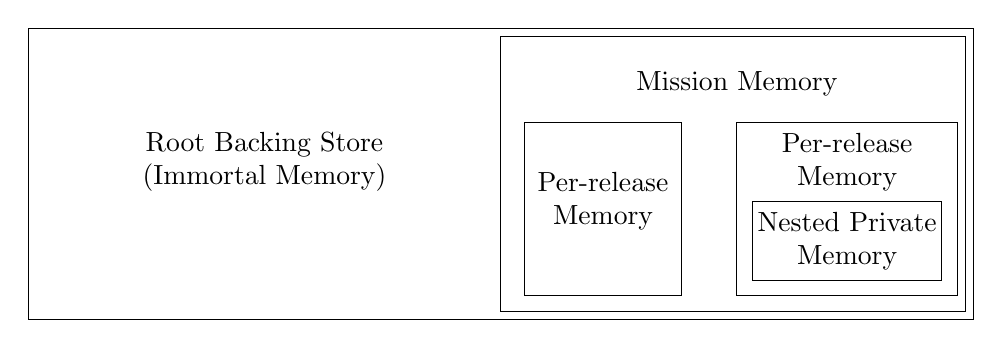
\begin{tikzpicture}
    \draw (0,0) rectangle (12,3.7);
    \node[align=center] at (3,2) {Root Backing Store\\(Immortal Memory)};
    
    \draw (6,0.1) rectangle (11.9,3.6);
    \node[align=center] at (9,3) {Mission Memory};
    
    \draw (6.3,0.3) rectangle (8.3,2.5);
    \node[align=center] at (7.3,1.5) {Per-release\\Memory};
    
    \draw (9,0.3) rectangle (11.8,2.5);
    \node[align=center] at (10.4,2) {Per-release\\Memory};
    
    \draw (9.2,0.5) rectangle (11.6,1.5);
    \node[align=center] at (10.4,1) {Nested Private\\Memory};
  \end{tikzpicture}
  \caption{An illustration of an example memory layout}
  \label{memory-fig}
\end{figure}

The operations of the memory manager API are summarised in
Table~\ref{memory-manager-table}. In addition to the inputs and outputs
described there, there should also be some system of reporting erroneous inputs,
whether that be exceptions, global error flags or particular return values
signalling errors. The conditions that cause an error to be reported are listed
in the final column of the table.

\begin{table}[ht]
  \centering
  \footnotesize
  \begin{tabular}{|l|p{3cm}|p{3cm}|p{3.6cm}|}
    Operation & Inputs & Outputs & Error Conditions \\
    \hline
    getRootBackingStore &
      (none) &
      backing store identifer &
      (none)
    \\getCurrentAllocationContext &
      (none) &
      backing store identifier &
      (none)
    \\setCurrentAllocationContext &
      backing store identifier &
      (none) &
      invalid identifier
    \\getTotalSize &
      backing store identifier &
      size in bytes &
      invalid identifier
    \\getUsedSize &
      backing store identifier &
      size in bytes &
      invalid identifier
    \\getFreeSize &
      backing store identifier &
      size in bytes &
      invalid identifier
    \\findBackingStore &
      memory pointer &
      backing store identifier &
      no backing store found
    \\allocateMemory &
      size in bytes &
      memory pointer &
      insufficient free memory
    \\makeBackingStore &
      size in bytes & 
      backing store identifier &
      insufficient free memory
    \\clearCurrentAllocationContext &
      (none) &
      (none) &
      nested backing store in use
    \\resizeBackingStore &
      backing store identifier \newline
      size in bytes &
      (none) &
      invalid identifier \newline
      insufficient free space \newline
      backing store is root \newline
      backing store not empty \newline
      backing store not only child
    \\createStack &
      size in bytes &
      stack identifier &
      insufficient free space
    \\destroyStack &
      stack identifier &
      (none) &
      invalid identifier
  \end{tabular}
  \caption{The operations of the SCJVM memory manager}
  \label{memory-manager-table}
\end{table}

The root backing store described above is always available to the SCJ
infrastructure through the \texttt{get\-Root\-Backing\-Store} operation. An SCJ
program does not have direct access to the root backing store except through
memory areas provided by the infrastructure.

In addition to managing the layout of backing stores in general, the memory
manager must also track what the current allocation context is. The operations
\texttt{get\-Cur\-rent\-Allo\-cation\-Con\-text} and
\texttt{set\-Cur\-rent\-Allo\-cation\-Con\-text} provide a means to get and set the
current allocation context. The functionality of changing the allocation context
is used by the methods of the SCJ API that allow code to be run with a different
memory area as allocation context, such as \texttt{execute\-In\-Area\-Of()} and
\texttt{enter\-Private\-Memory()}. The memory manager stores each thread's
allocation context and queries the scheduler as to which thread is current when
it performs operations affecting the current allocation context.

It is possible to obtain information about the used and available space in a given
backing store using the operations \texttt{get\-Total\-Size},
\texttt{get\-Used\-Size}, and \texttt{get\-Free\-Size}. This information is made
available to SCJ programs through the interface provided by memory areas.

Another query that can be made concerning backing stores is that of which
backing store a particular memory address lies in. This information can be
obtained by the \texttt{find\-Backing\-Store} operation and is required by the
infrastructure for obtaining the memory area of a given object.

Allocation within backing stores is possible through the
\texttt{allo\-cate\-Memory} operation, which allocates blocks of memory within
the current allocation context. This operation is provided in order for the core
execution environment to implement the \texttt{new} bytecode instruction and
should not be directly available to the program or infrastructure. Allocations
within backing stores must not cause fragmentation, so as to fulfil real-time
predictability requirements. The operation \texttt{allo\-cate\-Memory} must also
zero the memory it allocates, in order to properly match the semantics of
\texttt{new}.
 
Allocation of backing stores, which may require additional information attached
to them, is provided for by \texttt{make\-Back\-ing\-Store}, which is available
to the infrastructure for use when creating new memory areas. A new backing
store is created nested within the current allocation context. The
infrastructure is responsible for storing the backing store identifier returned
by the \texttt{make\-Backing\-Store} operation. The allocation of backing stores
is required to be done in constant time without fragmentation.

Deallocation of memory in backing stores cannot be done directly as that could
introduce fragmentation and would defeat the scoped memory model of
SCJ. Instead, the SCJVM provides for clearing a backing store when the memory
area it serves is no longer in use. This functionality is provided by the
operation \texttt{clear\-Current\-Allocation\-Context}, which clears the current
allocation context. It is not necessary to track exactly which object are
deallocated by this operation as SCJ does not have object finalisers. The
clearing of a backing store includes the clearing and removal of all backing
stores nested within it. This would create a problem if the parent backing store
is cleared while another thread is using a backing store within it as an
allocation context. However, such a situation should not occur as the backing
stores of mission memory and immortal memory are the only backing stores that
contain backing stores in use by different threads. Mission memory is only
cleared when all the event handler threads within the mission have finished and
immortal memory should never be cleared.

The last operation on backing stores is their resizing. This is provided for by
\texttt{resize\-Backing\-Store} but, as resizing a backing store presents a lot
of difficulties in terms of fragmentation, there are several restrictions. In
addition to being a valid backing store and there being enough space in the
parent backing store for the resizing to take place, a backing store to be
resized must not be the root backing store and must be empty and the only
backing store within its parent.  However, the only situations in which a
backing store resize is required are resizing of mission memory in between
missions and resizing of nested private memory when it is reentered. In both
these cases all the above points hold.

In addition to managing backing stores, the memory manager must also manage
stacks, which are placed in a separate area of memory to the backing stores. The
operations \texttt{create\-Stack} and \texttt{destroy\-Stack} allow for stacks
to be created and destroyed respectively. The stack space must not be fragmented
but this should not be an issue as stacks for threads are allocated together
when the mission is initialised and destroyed together when the mission
ends. That remains true at level 2 where nested missions are permitted as the
nested mission's stacks will be allocated after the stacks of it's parent
mission and will be destroyed before the parent mission ends. Like backing
stores, stacks are referred to by unique identifiers that may simply be pointers
to the space allocated for the stack.

\section{Scheduler API}
\label{scheduler-sec}

The SCJVM scheduler manages the scheduling of threads. The operations of the
scheduler are summarised in Table~\ref{scheduler-table}.

\begin{table}[ht]
  \centering
  \footnotesize
  \begin{tabular}{|l|p{3cm}|p{2.2cm}|p{2.7cm}|}
    Operation & Inputs & Outputs & Error Conditions \\
    \hline
    getMaxSoftwarePriority &
      (none) &
      priority level &
      (none)
    \\getMinSoftwarePriority &
      (none) &
      priority level &
      (none)
    \\getNormSoftwarePriority &
      (none) &
      priority level &
      (none)
    \\getMaxHardwarePriority &
      (none) &
      priority level &
      (none)
    \\getMinHardwarePriority &
      (none) &
      priority level &
      (none)
    \\getMainThread &
      (none) &
      thread identifier &
      (none)
    \\makeThread &
      entry point \newline
      priority level \newline
      backing store identifier \newline
      stack identifier &
      thread identifier &
      invalid priority \newline
      invalid backing store \newline
      invalid stack
    \\startThread &
      thread identifier &
      (none) &
      invalid identifier
    \\getCurrentThread &
      (none) &
      thread identifier &
      (none)
    \\destroyThread &
      thread identifier &
      (none) &
      invalid identifier
    \\suspendThread &
      (none) &
      (none) &
      (none)
    \\resumeThread &
      thread identifier &
      (none) &
      invalid identifier
    \\setPriorityCeiling &
      pointer to object \newline
      priority level &
      (none) &
      invalid priority
    \\takeLock &
      pointer to object &
      (none) &
      lock in use
    \\releaseLock &
      pointer to object &
      (none) &
      lock not held
    \\attachInterruptHandler &
      interrupt identifier \newline
      entry point &
      (none) &
      invalid interrupt
    \\detachInterruptHandler &
      interrupt identifier &
      (none) &
      invalid interrupt
    \\getInterruptPriority &
      interrupt identifier &
      priority level &
      invalid interrupt
    \\disableInterrupts &
      (none) &
      (none) &
      (none)
    \\enableInterrupts &
      (none) &
      (none) &
      (none)
  \end{tabular}
  \caption{The operations of the SCJVM scheduler}
  \label{scheduler-table}
\end{table}

Each thread is scheduled according to a priority level. The SCJ standard
requires that there be at least 28 priorities and separates them into hardware
and software priorities, with hardware priorities being higher than software
priorities. The range of priorities that a VM actually supports may vary between
different VM implementations within these restrictions. To allow the range of
supported priorities to be determined and support corresponding methods in the
SCJ API, the minimum and maximum hardware and software priority levels can be
obtained with \texttt{get\-Max\-Soft\-ware\-Pri\-or\-ity},
\texttt{get\-Min\-Soft\-ware\-Pri\-or\-ity},
\texttt{get\-Max\-Hard\-ware\-Pri\-or\-ity}, and
\texttt{get\-Min\-Hard\-ware\-Pri\-or\-ity}. The SCJVM chooses a default normal
software priority for threads, that can be queried through the
\texttt{get\-Norm\-Soft\-ware\-Pri\-or\-ity} operation.

Initially there is one thread running, which is called the main thread. The main
thread is created when the VM starts and has an implementation-defined
priority. The main thread can be suspended by the infrastructure when it is not
needed and resumed when it is needed again, using the operations mentioned
below. This allows it to be used for setting up the SCJ application and
missions, then suspended during mission execution. The main thread's identifier
can be retrieved using the \texttt{get\-Main\-Thread} operation.

Threads other than the main thread can be created by the \texttt{create\-Thread}
operation, which takes the entry point and priority level of the thread to be
created, as well as a backing store as the allocation context and a stack to use
for the thread. This operation returns the identifier of the newly created
thread, which must be stored by the infrastructure. The SCJVM does not
distinguish between the different thread release conditions so for
periodic and one-shot threads the infrastructure must set a timer separately
using the real-time clock API when a thread is created. The only priorities
allowed for threads are the software priorities, as hardware priorities are
reserved for interrupts. The backing store supplied here is only used to set the
backing store in the memory manager when the thread starts and is not stored by
the scheduler beyond that.

The SCJVM threads that are eligible to run must be scheduled as if they are
placed in queues with one queue for each priority. At each moment in time, the
thread at the front of the highest priority non-empty queue is running. A thread
becomes eligible to run after it is started and stops being eligible to run when
it is blocked. A thread is started using the \texttt{start\-Thread} operation
and must be started by the infrastructure when its enclosing mission starts. The
reason for the separation between thread creation and thread starting is to
ensure that threads all start together after mission initialisation has been
completely finished.

The identifier of the currently running thread can be obtained through the
\texttt{get\-Current\-Thread} operation. This operation may be used by the
infrastructure as part of obtaining the current schedulable object but is mainly
intended for use by the memory manager in order to discern what the current
allocation context is.

A thread can be suspended, causing it to become blocked, and resumed, causing it
to become eligible to run again, by the operations \texttt{suspend\-Thread} and
\texttt{resume\-Thread}. These operations are only visible to the program
through \texttt{wait()} and \texttt{notify()} at level 2. These operations are
also used in hardware communication, when a thread must wait for hardware to
complete a request, and to implement thread release, whereby a thread
remains suspended until released.

A thread that has been created can then be destroyed with the
\texttt{destroy\-Thread} operation, which removes the thread from the scheduler.
Destroying a thread does not automatically destroy its stack or the backing
store being used as its allocation context. The SCJ infrastructure should not
destroy a thread while it is running as a thread should only be destroyed when
the mission it is part of is ending. The infrastructure should instead ensure
that all threads in a mission are suspended before destroying them.

The SCJVM must support priority ceiling emulation, as it is required by
SCJ. This is handled by providing the \texttt{set\-Priority\-Ceiling} operation
that associates a priority ceiling value to an object identified by a
pointer. An object that does not have its priority ceiling explicitly set has a
priority ceiling equal to the default ceiling, which should be the highest
software priority but it is possible that a virtual machine could have an option
to change the default priority ceiling. Note that the SCJVM scheduler does not
require a notion of object in order to associate priority ceilings to objects as
the object's pointer can be used as an opaque identifier.

The operations for taking and releasing locks are \texttt{takeLock} and
\texttt{releaseLock}. A thread can only take a lock if its active priority and
the ceiling priorities of any other objects it holds the locks for is less than
or equal to the ceiling priority of the object the lock is being taken on. Only
one thread can take a given object's lock at a time. When a lock is taken, the
thread's active priority is raised to the object's priority ceiling. When a
thread releases a lock, the thread's active priority is lowered to its previous
active priority (the thread may hold nested locks on multiple objects).

The SCJVM scheduler must also manage interrupts, as interrupt handlers have
priorities (though these should be in the hardware priority range) and so must
be dealt with within the priority scheduling model. An interrupt handler can be
attached to a given interrupt using the \texttt{attach\-Interrupt\-Handler}
operation and an interrupt's handler can be removed with the
\texttt{detach\-Interrupt\-Handler} operation. An interrupt with no handler
attached to it is ignored. The clock interrupt coming from hardware is handled
by the SCJVM clock (see Section~\ref{realtime-clock-sec}) and converted into a
clock interrupt that is passed to the scheduler for handling by the attached
interrupt handler (which should simply call the \texttt{triggerAlarm()} method
of \texttt{Clock}).

Each interrupt has a priority associated with it, which is set by the SCJVM on
startup and cannot be changed by the application. These interrupt priorities
must be hardware priorities. An interrupt handler will interrupt any
lower-priority interrupt handler and any running threads, and blocks
lower-priority interrupt handlers from running until it has finished. The
priority associated with each interrupt can be obtained by the
\texttt{get\-Interrupt\-Priority} operation.

Interrupts can be disabled using the \texttt{disable\-Interrupts} operation and
re-enabled using the \texttt{enable\-Interrupts} operation. While interrupts are
disabled no interrupt handlers can run but it is implementation-defined as to
whether or not interrupts fired while interrupts are disabled are lost.

\section{Real-time Clock API}
\label{realtime-clock-sec}

The SCJVM must manage the system real-time clock, providing an interface that
allows for the time to be read and alarms to be set to trigger time-based
events. The operations of the SCJVM real-time clock are summarised in
Table~\ref{realtime-clock-table}.

\begin{table}[ht]
  \centering
  \footnotesize
  \begin{tabular}{|l|p{0.9cm}|p{1.8cm}|p{2.3cm}|}
    Operation & Inputs & Outputs & Error Conditions \\
    \hline
    getSystemTime &
      (none) &
      time &
      (none)
    \\getSystemTimePrecision &
      (none) &
      time precision &
      (none)
    \\setAlarm &
      time &
      (none) &
      time in past
    \\clearAlarm &
      (none) &
      (none) &
      (none)
  \end{tabular}
  \caption{The operations of the SCJVM real-time clock}
  \label{realtime-clock-table}
\end{table}

The main function of the real-time clock API is to provide access to the system
time through the \texttt{get\-System\-Time} operation. The SCJ API deals with
time values in terms of milliseconds-nanoseconds pairs, that should also be the
format for time values passed to and from the SCJVM though another format could
be used. The system time may be measured from January 1, 1970 or from the system
start time (in case there is no reliable means of determining the date
and time), and so may not correspond to wall-clock time.

The time between ticks of the system clock (its precision) must be made
available through the \texttt{get\-System\-Time\-Precision} operation. The
clock's precision must not change.

The SCJVM must also provide a facility to set an alarm that sends a clock
interrupt to the scheduler when a specific time is reached. This facility is
provided by the \texttt{set\-Alarm} function, which accepts an absolute time
value at which the alarm should trigger. The time passed to \texttt{set\-Alarm}
is required to not be in the past. Running code at a specified relative time
offset should be handled by the infrastructure. Once a alarm has triggered, it
is removed and a new alarm must be set in order to perform events periodically.

The current alarm (if any) can be cleared using the \texttt{clear\-Alarm}
operation.

\section{Formal Model}
\label{formal-model-section}

The formal model of the SCJVM is written in the \Circus{} specification
language~\cite{oliveira2009}. \Circus{} is based on CSP~\cite{roscoe2011}, which
is used to specify processes that communicate over channels, and the Z
notation~\cite{woodcock1996}, which is used to specify state and data
operations. In this section, we present a brief explanation of \Circus{} and an
overview of our model. We then present part of the memory manager model to to
show how it is constructed. The complete model can be found
in the appendix to this report. It is type checked with Community Z Tools and we have
started to prove some basic properties of the memory manager using Z/Eves.

A \Circus{} specification is made up of processes that communicate over
channels.  These channels may carry values of a particular type, or may be used
as flags for synchronisation or signalling between processes.  Each process may
have state, and is made up of actions that operate on that state and communicate
over channels.

In our model, each of the components of the SCJVM shown in
Figure~\ref{scjvm-fig} is specified by a single process whose channels represent
the services they provide.  The whole collection of VM services are then
specified by a parallel composition of the memory manager, scheduler and clock
processes. In this case, parallelism is being used to define a conjunction of
requirements. 

The processes synchronise on the channels they share, specified in the
sets $MMSInterface$ and $RTCSInterface$. The set $MMSInterface$ is the interface
between the memory manager and the scheduler, which contains a channel to get
the current thread from the scheduler, and channels to inform the memory manager
of the creation and destruction of threads. The interface between the real-time
clock and the scheduler, $RTCSInterface$, contains a channel to pass the clock
interrupt to the scheduler for handling. The channels used for internal
communication between the VM services are hidden so that the only channels that
can be used to communicate with the VM services are those used to represent the
services in Tables~\ref{memory-manager-table}, \ref{scheduler-table} and
\ref{realtime-clock-table}, and those used for communication with the core
execution environment.
%
\begin{circus}
  VMServices \circdef \\
  \t1 ((MemoryManager \lpar MMSInterface \rpar Scheduler) \\
  \t2 \lpar RTCSInterface \rpar RealtimeClock) \\
  \t3 \circhide VMServicesInternals
\end{circus}
%
The parallel composition of $VMServices$ with a process representing the core
execution environment (which, as mentioned, we do not specify here)
specifies the full SCJVM.

Our model of the scheduler is similar to other formal models of priority
schedulers~\cite{ferreira2014, gotsman2013, klein2014, lime2009}, and the
real-time clock specification is fairly simple and just manages the current time
and any alarm that may be set. For those reasons, we do not go into detail on
the scheduler on clock models here. Instead, we present part of the memory
manager model, which is the most complex of the three VM services.  We show the
memory manager state and some of the operations. We also explain how the formal
specification reflects the requirements identified in
Section~\ref{memory-manager-sec}.

The memory manager specification begins by declaring a type, $MemoryAddress$, of
memory addresses to be the set of natural numbers.  This then allows for
specification of a type, $ContiguousMemory$, that contains contiguous ranges of
memory addresses and is used to specify that backing stores must not be
fragmented.
%
\begin{zed}
	MemoryAddress == \nat \\
	ContiguousMemory == \\
        \t1 \{~ m : \power MemoryAddress | \\
        \t2 \exists a, b : MemoryAddress @ m = a \upto b ~\}
\end{zed}
%
Backing stores are identified by identifiers that are elements of a type
$BackingStoreID$. These are simply opaque identifiers and there are no
constraints on $BackingStoreID$ beyond the fact that it exists.

We specify backing stores in two parts. The first part, $MemoryBlock$, stores
the used, free and total memory and allows for allocation within it. This aspect
of backing stores is separated out because it is also used in specifying the
stack space, since allocation of memory also occurs there.The variables $used$
and $free$ correspond to the areas of used and free memory, while $total$
represents the whole memory area covered by the $MemoryBlock$. Note that $free$
and $total$ are required to be contiguous to enforce the requirement that there
must be no fragmentation whereas it is not necessary that $used$ is simply
specified to be a set of memory addresses. There are two invariants on
$MemoryBlock$, identified by the predicates in the schema above. The first
invariant simply specifies that $used$ and $free$ must be contained in $total$,
but it does not require them to cover $total$ as there may be some additional
memory overhead. The second invariant requires $used$ and $free$ to be disjoint.
%
\begin{schema}{MemoryBlock}
  free, total : ContiguousMemory \\
  used : \power MemoryAddress \\
\where
  used \cup free \subseteq total \\
  used \cap free = \emptyset \\
\end{schema}
%
A $MemoryBlock$ is initialised by the $MemoryBlockInit$ operation, which accepts
as an input a contiguous area of memory, $addresses?$, that it should cover. The
final state of the operation is represented by variables obtained by placing a
prime on the names of the state components. The variable $total'$ is specified
to be equal to $addresses?$ and $used'$ is specified to be empty. The variable
$free'$ is permitted to take any value, provided that it is a subset of
$addresses?$.
%
\begin{schema}{MemoryBlockInit}
  MemoryBlock~' \\
  addresses? : ContiguousMemory \\
\where
  total' = addresses? \\
  free' \subseteq addresses? \\
  used' = \emptyset \\
\end{schema}
%
As an example of an operation on $MemoryBlock$, we present $MBAllocate$, the
operation of allocating memory within a $MemoryBlock$. This operation takes an
input $size?$ that is the requested size of the allocated memory, and outputs an
area of contiguous memory called $allocated!$. There is a precondition on this
operation that $size?$ must be smaller than the size of $free$, to ensure that
there is enough free space to fulfil the allocation request. The output,
$allocated!$, is then specified to be of the requested size and contained within
$free$. The final state $used'$ is obtained by adding $allocated!$ to $used$ and
$free'$ is obtained by removing $allocated!$ from $free$. Finally, it is
specified that $total$ does not change.
%
\begin{schema}{MBAllocate}
  \Delta MemoryBlock \\
  size? : \nat \\
  allocated! : ContiguousMemory
\where
  size? \leq \# free \\
  \# allocated! = size? \land allocated! \subseteq free \\
  used' = used \cup allocated! \\
  free' = free \setminus allocated! \\
  total' = total \\
\end{schema}
%
With $MemoryBlock$ specified, the remaining parts of the backing store state are
added in the schema $BackingStore$, which is a $MemoryBlock$ with a variable,
$self$, to store its own identifier and a finite set, $children$, of the
identifiers of its immediate children. The invariants specify that it cannot be
a child of itself and that the overhead, left loosely specified in
$MemoryBlock$, must have a size equal to some constant
$backingStoreOverhead$. The invariants inherited from $MemoryBlock$ are also
required to hold.
%
\begin{schema}{BackingStore}
	MemoryBlock \\
  	self : BackingStoreID \\
  	children : \finset BackingStoreID \\
\where
 	self \notin children \\
 	\# total = \\
        \t1 \# used + \# free + backingStoreOverhead
\end{schema}
%
Initialisation of a $BackingStore$ is handled by the operation
$BackingStoreInit$, which behaves as $MemoryBlockInit$ with the additional
precondition that the size $addresses?$ must be larger than
$backingStoreOverhead$ and the requirement that $free'$ be made smaller than
$addresses?$ to allow space for $backingStoreOverhead$. For the new state
components, $self'$ is specified by an additional input $newID?$ and $children'$
is specified to be empty.
\begin{schema}{BackingStoreInit}
  BackingStore~' \\
  MemoryBlockInit \\
  newID? : BackingStoreID \\
\where
  \# addresses? \geq backingStoreOverhead \\
  \# free' = \# addresses? - backingStoreOverhead \\
  self' = newID? \\
  children' = \emptyset \\
\end{schema}
%
An example of a $BackingStore$ operation is allocating space for a new child
backing store within its parent. That operation is given by the the schema
$BSAllocateChild$ below.
%
\begin{schema}{BSAllocateChild}
  \Delta BackingStore \\
  MBAllocate \\
  childID! : BackingStoreID \\
  \where
  childID! \notin children \land childID! \neq self \\
  children' = children \cup \{ childID! \} \\
  self' = self
\end{schema}
%
This operation is based on $MBAllocate$, but it has an additional output,
$childID!$, which is the identifier of the newly allocated child, and it
specifies how the extra state components in $BackingStore$ are updated. The new
child's identifer is specified to not be the identifier of an existing child and
must not be the identifier of the backing store itself. The final state
$children'$ is specified to add $childID!$ to $children$ and $self$ does not
change. This operation is made into a robust operation, $RBSAllocateChild$, that
handles the case where the precondition does not hold by outputting a value
$report!$, which is either a reported error or the value $okay$.

Backing stores are managed by the global memory manager, the state of which is
given by the schema below. The global memory manager state contains a partial
function, $stores$, that relates backing store identifiers to the backing
stores, along with the identifier, $rootBackingStore$, of the root backing store
and a relation, $childRelation$ between backing store identifiers and the
identifiers of their direct children. The global state also contains a map,
$threadACs$, from thread identifiers to their allocation context, which is used,
together with information obtained from the scheduler, to perform operations on
the current allocation context.

The relationships between the backing stores are specified by the invariants of
this state as defined by the predicates in the schema above. The first invariant
specifies that the root backing store must be a valid identifier (this is
implied by the sixth invariant but is written separately for clarity). The
second invariant is an injectivity condition on $stores$, requiring that no two
backing stores have the same identifier. The third invariant requires that a
backing store's childres are all disjoint and contained in that backing store's 
used memory. The fourth invariant requires that
the thread allocation contexts be valid backing stores. The fifth invariant 
defines $childRelation$, using the set of children in the backing store record
to form a relation between backing store identifiers. The sixth invariant uses
the reflexive transitive closure of $childRelation$ to specify that every known
backing store must be a (direct or indirect) child of the root backing store or
the root backing store itself. Lastly, the seventh invariant specifies that no
backing store can be a (direct or indirect) child of itself.
%
\begin{schema}{GlobalMemoryManager}
  stores : BackingStoreID \pfun BackingStore \\
  childRelation : \\
    \t1 BackingStoreID \rel BackingStoreID \\
  rootBackingStore : BackingStoreID \\
  threadACs : ThreadID \pfun BackingStoreID \\
\where
  rootBackingStore \in \dom~stores \\
  \forall b: \dom~stores @ (stores~b).self = b \\
  \forall b : \ran stores @ \exists m : \power b.used @ \\
    \t1 (\lambda x : b.children @ (stores~x).total) \\
    \t2 \partition m \\
  \ran threadACs \subseteq \dom stores \\
  childRelation = \bigcup \{ i : \dom~stores @ \\ 
    \t1 \{ j : (stores~i).children @ (i,j) \} \} \\
  \dom stores = \\
    \t1 (childRelation\star) \limg \{ rootBackingStore \} \rimg \\
  \forall s : \dom stores @ s \notin childRelation\plus \limg \{ s \} \rimg \\
\end{schema}
%
The operations on the memory manager are specified using the Z idiom of
promotion, which allows operations on a local state to be lifted to operations on
a global state.  This allows simple operations on the backing store records to be
used to update the backing stores in the $stores$ function.  As an
example we present the $GlobalMakeBS$ schema that specifies the creation of a
backing store within another.

Much of this operation's complexity comes from the fact that it is
promoting two operations: $RBSAllocateChild$ and $BackingStoreInit$. The
allocation occurs in the current allocation context, identified by the input
$allocationContext?$. It is determined by obtaining the current thread from the
scheduler, looking up its allocation context and passing it as an input to the
operation specified by the Z schema.

The first condition on the operation requires that the allocation context be a
valid backing store, that is, in the domain of $stores$. After that, the
existential quantifiers introduce variables local to the schema, specifying the
size of the allocated backing store, $actualSize$, to include some
implementation-defined overhead.

Then the promotions are specified, beginning with the operation
$RBSAllocateChild$. The local variables $childID!$ and $childAddresses!$ are
identified with outputs of the promoted operation that have the same names. The
initial state for the promoted operation is taken from the backing store in
$stores$, and the final state is placed in the variable $parent$.  The output
$childID!$ is required to not be the identifier of another backing store. It is
required that no error be reported in the error reporting variable $report!$.

The second operation promoted is $BackingStoreInit$. The variables
$actualSize$, $childAddresses!$ and $childID!$ are passed to it as inputs via
renaming. The final state of the promoted operation is stored in $child$.  The final 
states of both backing stores, $parent$ and $child$ are stored in the $stores$
function, with $childID!$ being used as the identifier of $child$. The 
specification of the operation ends by stating that all other state variables
remain the same.
%
\begin{schema}{GlobalMakeBS}
  \Delta GlobalMemoryManager \\
  size? : \nat \\
  allocationContext? : BackingStoreID \\
\where
  allocationContext? \in \dom stores \\
  \exists actualSize : \nat | \\
  \t1 actualSize = size? + backingStoreOverhead @ \\
  \exists childID! : BackingStoreID @ \\
  \exists allocated! : ContiguousMemory @ \\
  \exists parent, child : BackingStore @ \\
  \t1 (\exists \Delta BackingStore; report! : Report | \\
    \t2 RBSAllocateChild [ actualSize / size? ] @ \\
    \t2 \theta BackingStore = \\
      \t3 stores~allocationContext? \land \\
    \t2 parent = \theta BackingStore~' \land \\
    \t2 childID! \notin \dom stores \land \\
    \t2 report! = okay) \land \\
  \t1 (\exists BackingStore~'; report! : Report | \\
    \t2 BackingStoreInit [ allocated! / addresses? ] @ \\
    \t2 child = \theta BackingStore~') \land \\
  \t1 stores' = stores \oplus \\
    \t2 \{ allocationContext? \mapsto parent, \\
    \t2 childID! \mapsto child \} \\
  rootBackingStore' = rootBackingStore \\
  childRelation' = childRelation \\
  threadACs' = threadACs \\
\end{schema}
%
Other global memory manager operations are similarly specified using
promotion. Operations on stacks are specified separately, using a
specification based on $MemoryBlock$.

\chapter{Conclusions}
\label{conclusions-chapter}

% Similar to JTRES paper conclusions

\raggedright
\printbibliography
\end{document}
